\section{SimSite3D::rigid\_\-align\_\-t Class Reference}
\label{classSimSite3D_1_1rigid__align__t}\index{SimSite3D::rigid_align_t@{SimSite3D::rigid\_\-align\_\-t}}
Data class: Holds the numerous features of an alignment.  


{\tt \#include $<$Score\-Map\-Base.H$>$}

Inheritance diagram for SimSite3D::rigid\_\-align\_\-t::\begin{figure}[H]
\begin{center}
\leavevmode
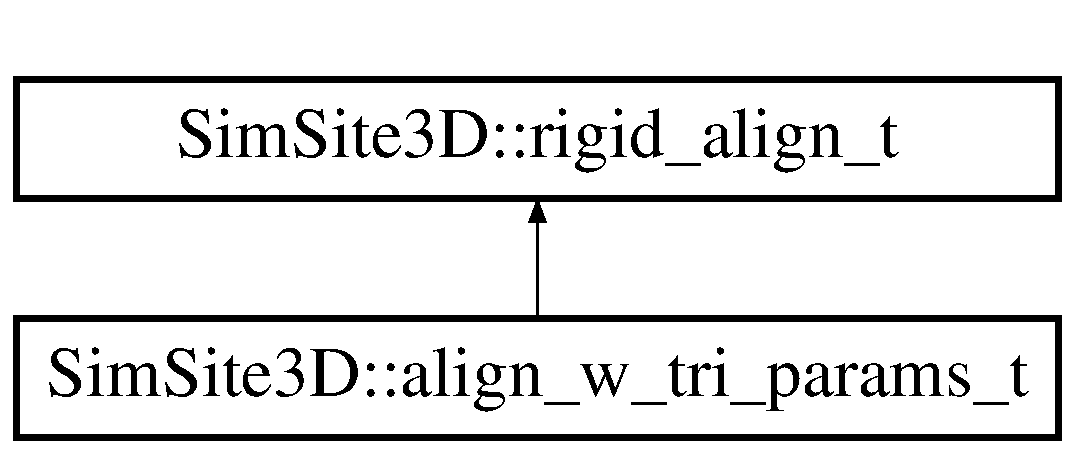
\includegraphics[height=2cm]{classSimSite3D_1_1rigid__align__t}
\end{center}
\end{figure}
\subsection*{Public Member Functions}
\begin{CompactItemize}
\item 
\bf{rigid\_\-align\_\-t} ()\label{classSimSite3D_1_1rigid__align__t_e6335cc41892b44aba75afb30c42422b}

\begin{CompactList}\small\item\em Initialize the features to zero or very large values. \item\end{CompactList}\item 
\bf{rigid\_\-align\_\-t} (const \bf{rigid\_\-align\_\-t} \&other)\label{classSimSite3D_1_1rigid__align__t_e05610ac44e3120513667837de227445}

\begin{CompactList}\small\item\em Basic copy constructor. \item\end{CompactList}\item 
const \bf{rigid\_\-align\_\-t} \& \bf{operator=} (const \bf{rigid\_\-align\_\-t} \&other)\label{classSimSite3D_1_1rigid__align__t_e42d7414871c06710daf9f23d71d349d}

\begin{CompactList}\small\item\em Basic assignment operator. \item\end{CompactList}\item 
virtual \bf{$\sim$rigid\_\-align\_\-t} ()\label{classSimSite3D_1_1rigid__align__t_be237ac53c1d6917a5ff2c717574b955}

\begin{CompactList}\small\item\em Do nothing destructor. \item\end{CompactList}\item 
bool \bf{operator==} (const \bf{rigid\_\-align\_\-t} \&b) const 
\item 
bool \bf{operator!=} (const \bf{rigid\_\-align\_\-t} \&b) const 
\item 
virtual void \textbf{write\_\-score\_\-fields} (std::ostream \&out, const uint orient\_\-num, const bool wrote\_\-ligs, const std::string \&ext\_\-SF\_\-id\_\-in, const std::string \&struct\_\-id, const std::string \&lig\_\-id) const \label{classSimSite3D_1_1rigid__align__t_12c292600e42cb9e61a87201d38b574d}

\item 
virtual void \textbf{write\_\-score\_\-fields} (std::ostream \&out) const \label{classSimSite3D_1_1rigid__align__t_c02636bc474643f5ceb468212ce470db}

\item 
virtual void \textbf{get\_\-score\_\-field\_\-labels} (std::vector$<$ std::string $>$ $\ast$fields, const bool normalize\_\-score) const \label{classSimSite3D_1_1rigid__align__t_c276978bf665b4f8899893f929333acf}

\item 
virtual void \textbf{set\_\-prot\_\-lig\_\-scores} (const my\_\-float\_\-t affiscore, const my\_\-float\_\-t orientscore, const my\_\-float\_\-t ligand\_\-efficiency)\label{classSimSite3D_1_1rigid__align__t_ab98b09f549c3700c63a772e495c8858}

\item 
virtual void \textbf{set\_\-triangle\_\-params} (const my\_\-float\_\-t perimeter, const my\_\-float\_\-t long\_\-len, const my\_\-float\_\-t short\_\-len)\label{classSimSite3D_1_1rigid__align__t_46db34052a8e92e8b9455b4d3adc4fa4}

\item 
virtual void \textbf{set\_\-number\_\-of\_\-orientations} (const size\_\-t num)\label{classSimSite3D_1_1rigid__align__t_482bac50e100ac69fb62edd5b3ff6775}

\item 
virtual void \textbf{save\_\-rigid\_\-alignment\_\-vals} ()\label{classSimSite3D_1_1rigid__align__t_b05738bb2695109d10c7b553ac7b4e42}

\item 
virtual void \textbf{save\_\-pre\-IK\_\-vals} ()\label{classSimSite3D_1_1rigid__align__t_8d323747e24f9374c1a94b364c3c415d}

\item 
virtual bool \textbf{compute\_\-prot\_\-lig\_\-score} ()\label{classSimSite3D_1_1rigid__align__t_b14c62f28834c0c953753b108954052e}

\item 
virtual void \textbf{set\_\-site\_\-atomic\_\-rmsd} (const my\_\-float\_\-t rmsd, const size\_\-t rmsd\_\-type)\label{classSimSite3D_1_1rigid__align__t_7f27991120704fa2a19cb8a7cf31ce55}

\end{CompactItemize}
\subsection*{Public Attributes}
\begin{CompactItemize}
\item 
my\_\-float\_\-t \bf{tier1\_\-score}\label{classSimSite3D_1_1rigid__align__t_1fef21d1eb205408a96f533891e79557}

\begin{CompactList}\small\item\em SimSite3D fast orientation score (sieve). \item\end{CompactList}\item 
my\_\-float\_\-t \bf{score}\label{classSimSite3D_1_1rigid__align__t_90a54e487c78c50e21dcb7f781cc37ef}

\begin{CompactList}\small\item\em Final SimSite3D score -- tier2. \item\end{CompactList}\item 
std::vector$<$ my\_\-float\_\-t $>$ \textbf{terms}\label{classSimSite3D_1_1rigid__align__t_6cf98bc92eac939ebe592ae47a49446a}

\item 
std::vector$<$ my\_\-float\_\-t $>$ \bf{ext\_\-scores}\label{classSimSite3D_1_1rigid__align__t_0ce6360ea3d61818cd088f34f2cf118d}

\begin{CompactList}\small\item\em External score(s). \item\end{CompactList}\item 
std::vector$<$ bool $>$ \textbf{frag\_\-atoms\_\-flags}\label{classSimSite3D_1_1rigid__align__t_8a3efbcef870f53faa51a54e64918e17}

\item 
my\_\-float\_\-t \bf{R} [9]\label{classSimSite3D_1_1rigid__align__t_c19150913ee8369262f89abf3dba1839}

\begin{CompactList}\small\item\em Rotation matrix for search to query. \item\end{CompactList}\item 
my\_\-float\_\-t \bf{T} [3]\label{classSimSite3D_1_1rigid__align__t_c66d5098258a0e0296c47b3d438dfd40}

\begin{CompactList}\small\item\em Translation vector for search to query. \item\end{CompactList}\item 
Quaternion \textbf{Q}\label{classSimSite3D_1_1rigid__align__t_ffd3c5b8182230bf24cc1ae954039360}

\item 
\bf{mol2File} $\ast$ \bf{frag\_\-file}\label{classSimSite3D_1_1rigid__align__t_be34b21f5d3ef687d3e9213aca149eb6}

\begin{CompactList}\small\item\em Pointer to the ligand fragment in query pocket. \item\end{CompactList}\item 
std::vector$<$ bool $>$ \textbf{match\_\-print}\label{classSimSite3D_1_1rigid__align__t_21450c7e527409561c1eaee7f46bf922}

\item 
my\_\-float\_\-t \textbf{hb\_\-caps\_\-score}\label{classSimSite3D_1_1rigid__align__t_956a632cdccaa9096759d9c1d38c6026}

\item 
std::string \textbf{hb\_\-caps\_\-match\_\-print}\label{classSimSite3D_1_1rigid__align__t_bd736c82ab7b0c5704c58fd85ca836a1}

\end{CompactItemize}
\subsection*{Private Member Functions}
\begin{CompactItemize}
\item 
void \textbf{init} ()\label{classSimSite3D_1_1rigid__align__t_19b9ab1fc878784b26ed6bf7a5d2338f}

\item 
void \bf{do\_\-copy} (const \bf{rigid\_\-align\_\-t} \&other)\label{classSimSite3D_1_1rigid__align__t_ab8efcf8e3820a7e91cd135acef58c84}

\begin{CompactList}\small\item\em A straightforward copy method. \item\end{CompactList}\end{CompactItemize}


\subsection{Detailed Description}
Data class: Holds the numerous features of an alignment. 

This class was supposed to make it easier to swap things in and out. However, it was put together relatively quickly and its major design flaw is that one cannot pick and choose score fields. It might be useful for future development if one can pick and choose pieces for scoring and reporting. 



\subsection{Member Function Documentation}
\index{SimSite3D::rigid_align_t@{SimSite3D::rigid\_\-align\_\-t}!operator"!=@{operator"!=}}
\index{operator"!=@{operator"!=}!SimSite3D::rigid_align_t@{SimSite3D::rigid\_\-align\_\-t}}
\subsubsection{\setlength{\rightskip}{0pt plus 5cm}bool SimSite3D::rigid\_\-align\_\-t::operator!= (const \bf{rigid\_\-align\_\-t} \& {\em b}) const\hspace{0.3cm}{\tt  [inline]}}\label{classSimSite3D_1_1rigid__align__t_dd0fdb2785fd9d00e710d9afd3253f4a}


Two alignments are not equal if their score is not the same or they do not have the same transformation \index{SimSite3D::rigid_align_t@{SimSite3D::rigid\_\-align\_\-t}!operator==@{operator==}}
\index{operator==@{operator==}!SimSite3D::rigid_align_t@{SimSite3D::rigid\_\-align\_\-t}}
\subsubsection{\setlength{\rightskip}{0pt plus 5cm}bool SimSite3D::rigid\_\-align\_\-t::operator== (const \bf{rigid\_\-align\_\-t} \& {\em b}) const\hspace{0.3cm}{\tt  [inline]}}\label{classSimSite3D_1_1rigid__align__t_3f01290c1017cdf9f9e1e6a3bf7af5ac}


Two alignments are equal if their score is the same and they have the same transformation 

The documentation for this class was generated from the following files:\begin{CompactItemize}
\item 
Score\-Map\-Base.H\item 
Score\-Map\-Base.C\end{CompactItemize}
